%!TEX root=../mythesis.tex
% Chapter Template

\chapter{Query Expansion} % Main chapter title
\chaptermark{Query Expansion}  % replace the chapter name with its abbreviated form
\label{ch:query_expansion}

%
In this chapter, we describe our final yet most significant contribution, \emph{query expansion}.
%
First, we introduce four main lines of related research in NLP that inspire our idea, namely \emph{attention mechanism}, \emph{synthetic data generation}, \emph{unsupervised pre-training} and \emph{query augmentation}.
%
We then move on to describe in detail our pipelined query expansion approach.
%
Finally, we discuss experimental results in which our proposed paradigm outperforms state-of-the-art approaches in OpenQA by substantial margins.


\section{Related Work}
\label{sec:query_expansion_related_work}


\begin{figure}[!htbp]
	\centering
	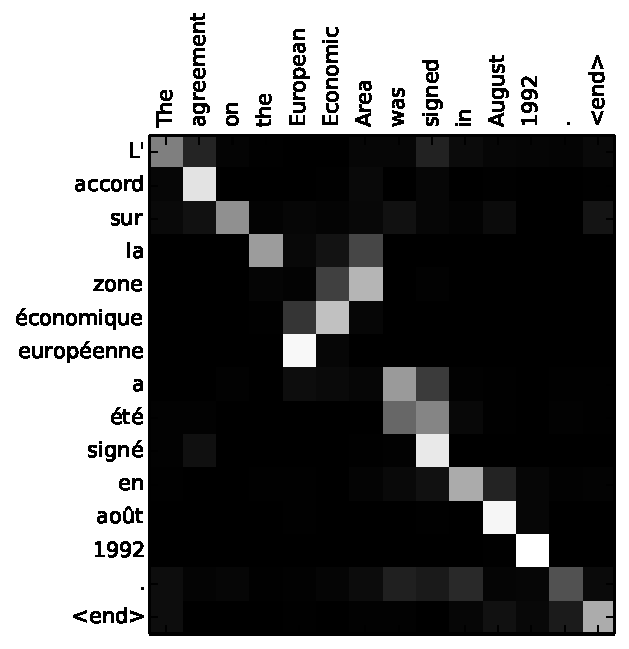
\includegraphics[width=0.6\linewidth]{query_expansion/attention_matrix_example.pdf}
	\caption[Illustration of the attention mechanism via the score matrix of an attention-based neural machine translation model.]{
		%
		An attention matrix $M$ of an attention-based neural machine translation model corresponding to a translation from English (x-axis) to French (y-axis).
		%
		Each cell $M_{ij}$ denotes the importance of the $j$-th word in the source sentence when the model is producing the $i$-th word in the target sentence, with white being the highest score and black being the lowest score.
		%
		We can observe that most of the time the model only looked at a few source words while ignoring the rest, and that the there is a linear alignment between the source and the target texts.
		%
		Interestingly, the entity \emph{European Economic Area} was translated to \emph{zone économique européenne} in French in a reverse direction, evidently shown by the attention matrix.
	}
	\label{fig:attention_illustration}
\end{figure}


\subsection{Attention Mechanism}
\label{sec:related_attention}

%
Early work in neural machine translation~\cite{luong2015effective, bahdanau2014neural} revealed and refined a novel soft alignment technique called \emph{attention}, which becomes a significant contribution in NLP and lays the foundation for many recent advances in natural language processing~\cite{vaswani2017attention, devlin2019bert}, computer vision~\cite{dosovitskiy2020image, liu2021swin} and reinforcement learning~\cite{tang2020neuroevolution, shen2019self}.
%
The attention mechanism is proposed to mimic the excellent human capability of paying attention only to the relevant parts when presented with a piece of information (e.g., an image or a text passage).
%
The idea is to guide the model to focus on those small but important pieces of evidence as it reads in the input sequence.
%
This can be best illustrated using an example in~\fref{fig:attention_illustration}.
%
Each cell $M_{ij}$ in the attention matrix denotes attention scores of a neural machine translation model assigning to the $j$-th word in the source sentence when translating the $i$-th word in the target sentence.
%
It is clear that most of the time, the model only looked at a single word in the source sentence that is one-to-one translated to the words in the target sentence.
%
By employing the attention mechanism, the model is allowed to ignore certain parts of the input sequence that are deemed irrelevant, and instead focus on relevant ones.
%
It is important to highlight that the attention mechanism has become ubiquitous in deep learning recently due to the tremendous performance gain it brings about with little extra computational cost, and has transformed into many variants such as self-attention or cross-attention.
%
We advance these observations one step further and propose a technique that takes advantage of cross-attention scores in an unsupervised manner to extract salient keywords from texts, which will be described later in~\sref{sec:query_expansion_method}.


\subsection{Synthetic Data Generation}


Synthetic data approaches aim at generating a set of artificially synthesized samples from the real, original data while trying to retain as much statistical distribution of the original data as possible.
%
Synthetic data generation has become increasingly predominant in the deep learning research community~\cite{wang2019learning, tripathi2019learning, lacoste2020synbols}, especially in the domains where the data is scarce such as medical treatment~\cite{chen2021synthetic, frid2018synthetic}.
%
Over the past decade, numerous synthetic data generation techniques have been proposed to tackle many aspects of machine learning, from early forms such as data augmentation~\cite{shorten2019survey, tran2017bayesian} or computer simulation~\cite{richter2016playing, song2017semantic} to more recent advances such as Generative Adversarial Networks (GANs)~\cite{goodfellow2014generative, karras2020analyzing} or pseudo data generation~\cite{arazo2020pseudo, wang2020unsupervised}.
%
Existing work in OpenQA adopted synthetic answer generation and question generation to improve the performance of existing state-of-the-art models in two main ways: \emph{unsupervised pre-training} and \emph{query augmentation}.


\subsection{Unsupervised Pre-training}
\label{sec:unsupervised_pre_training}


\begin{figure}[!ht]
	\centering
	
	\subfloat[Masked Language Modeling (Masked LM)]{%
		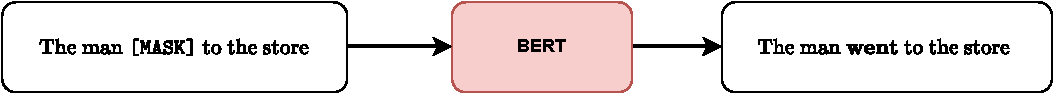
\includegraphics[clip,width=0.8\columnwidth]{query_expansion/masked_lm.pdf}%
	}
	\vspace{0.5cm}
	
	\subfloat[Next Sentence Prediction (NSP)]{%
		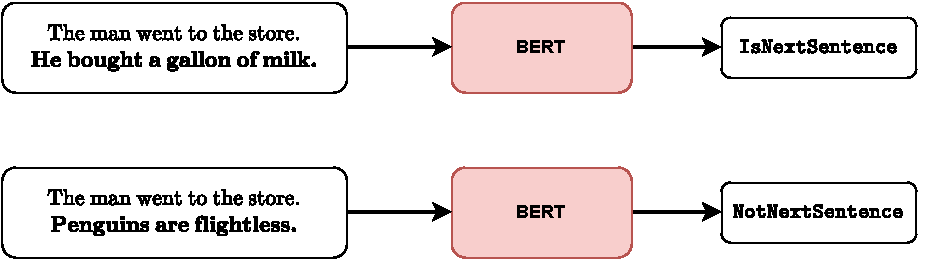
\includegraphics[clip,width=0.7\columnwidth]{query_expansion/next_sentence_prediction.pdf}%
	}
	\caption[BERT~\cite{devlin2019bert} unsupervised training objectives.]{
		%
		BERT~\cite{devlin2019bert} unsupervised training objectives.
		%
		With Masked LM, the model is asked to predict words that have been masked out of the sentence.
		%
		With Next Sentence Prediction, the model is asked to predict if a sentence is the grammatically and semantically possible next sentence of another sentence.
	}
	\label{fig:unsupervised_pretraining_bert}
\end{figure}


%
Together with the attention mechanism, \emph{unsupervised pre-training} has become a must-have recipe in natural language processing that contributes to recent rapid development in the field.
%
It all starts from the paper~\citet{devlin2019bert} which proposed to pre-train deep bidirectional transformer~\cite{vaswani2017attention} models on large unlabeled corpora of texts such as Wikipedia or Common Crawl.
%
In unsupervised pre-training, we are supplied with huge corpora of texts that can be easily crawled from the Internet, from which the models are required to perform natural language reasoning and understanding without any supervision.
%
This is made possible by carefully designed unsupervised objective functions, namely \emph{Masked Language Model} (Masked LM) and \emph{Next Sentence Prediction} (NSP).
%
\fref{fig:unsupervised_pretraining_bert} present illustrative examples of input-output pairs of the unsupervised training paradigm.
%
In Masked LM, a portion of the input text sequence is masked out using a special token $\texttt{[MASK]}$, for which the model is trained to predict the correct corresponding unmasked words.
%
On the other hand, Next Sentence Prediction takes a pair of consecutive sentences and randomly replaces the second sentence with another random sentence from the corpus.
%
The model is then trained to classify whether the latter sentence reasonably comes after the former sentence.
%
Importantly, unsupervised pre-training play a crucial role in many recent successes in deep learning~\cite{devlin2019bert, brown2020language, caron2020unsupervised, goyal2021self}, especially in the era of big data where unlabeled data can be obtained with virtually no effort.


\paragraph{Synthetic data training/pre-training}
%
In OpenQA, pre-training models with synthetic corpora has attracted increasing attention from researchers recently because it allows to observe much larger, more diverse datasets to improve model generalizability and performance.
%
\citet{alberti2019synthetic} used a sequence-to-sequence~\cite{sutskever2014sequence} model to generate synthetic questions from passages and a reading comprehension model to verify question answerability.
%
\citet{lewis2019unsupervised} sampled random nouns or entities from passages to generate a synthetic dataset of fill-in-the-blank cloze questions, which are then translated to natural questions using an unsupervised neural machine translation model.
%
This work showed that models trained on only synthetic data are able to achieve decent performance, testifying to the usability of generated data.
%
\citet{lewis2021paq} introduced a huge dataset of 65 million synthetic question-answer pairs using a sophisticated data generation pipeline.
%
A simple QA-pair retriever model trained on this dataset is able to match the performance of a two-stage retriever-reader model while being significantly faster.
%


\subsection{Query Augmentation}
%
In OpenQA, query augmentation techiques aim at preempting the query questions with relevant information, thus are expected to improve the retrieval stage substantially.
%
This technique is especially useful for multi-hop retrieval which requires information aggregation and complex reasoning over multiple pieces of evidence.
%
Given an input question, instead of trying to retrieve seemingly-unrelated related documents, we can enrich the query with relevant keywords retrieved from a pre-cached parametric memory.
%
It is important to note that to possibly incorporate all question-keywords pairs of a knowledge base to such memory, one must train a sequence-to-sequence model on a generated synthetic dataset that sufficiently covers all relationships within the knowledge base.
%
\citet{qi2019answering} proposed to iteratively enrich the query with progressively obtained keywords from previous steps to tackle the task of multi-hop open-domain question answering.
%
\citet{mao2021generation} demonstrated the advantages of query augmentation by performing only sparse retrieval using augmentated queries, achieving comparable performance as more computationally costly dense retrieval methods.

%
In this work, we take advantage of a huge synthetic question answering dataset for both synthetic data pre-training and query augmentation, which we will describe in detail in \sref{sec:query_expansion_method}.



\section{Method}
\label{sec:query_expansion_method}


\begin{figure}[!htbp]
	\centering
	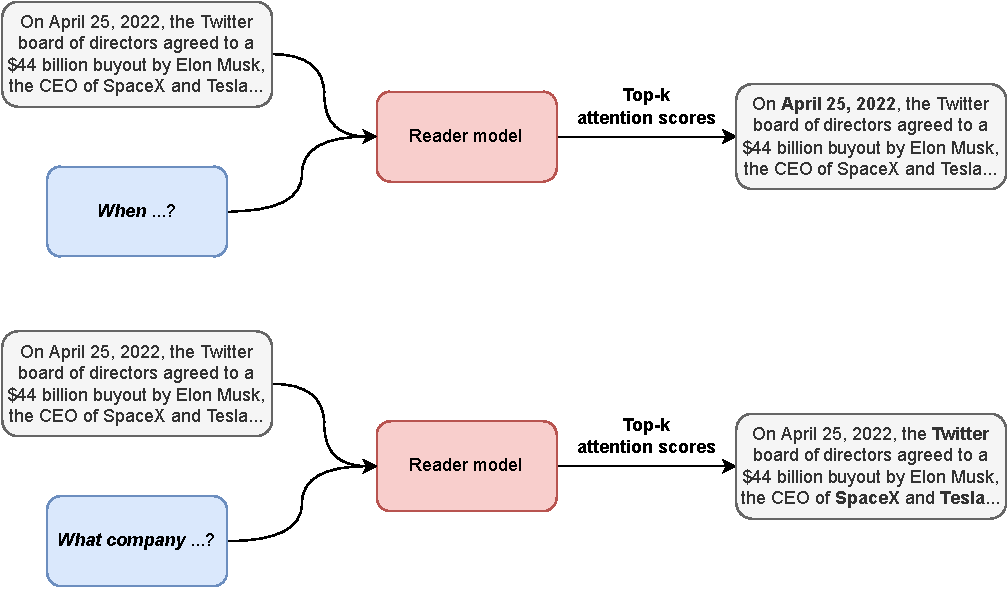
\includegraphics[width=0.95\linewidth]{query_expansion/question_type_specific.pdf}
	\caption[Illustration of the idea of unsupervised keyword extraction.]{
		%
		Illustration of the idea of unsupervised keyword extraction using a trained reader model.
		%
	 	When presented with a \emph{when} question, the model pays most attention to timestamps in the input passage (e.g., \emph{Apr 25, 2022}).
	 	%
	 	On the other hand, the model answer to a \emph{what company} question by attending to company names in the same input passage (e.g., \emph{Twitter}, \emph{SpaceX}, and \emph{Tesla}).
	}
	\label{fig:unsupervised_keyword_extraction}
\end{figure}


\subsection{Unsupervised Keyword Extraction}
\label{sec:unsupervised_keyword_extraction}
%
In this step, we generate salient keywords from passages in an unsupervised manner by exploiting attention scores as described in~\sref{sec:related_attention}.
%
This process is motivated by the observation that when generating an answer to a question, the generative reader model must pay attention to question type-specific tokens in the given relevant context passages.
%
\fref{fig:unsupervised_keyword_extraction} illustrates this idea, from which we observe that the model considers different sets of keywords highly depedent on the input question type.

%
In particular, suppose we have a large corpus $\mathcal{C}$ of $K$ factual documents $\{p_1, p_2, \ldots, p_K\}$, e.g., Wikipedia.
%
Furthermore, we are given a trained generative reader $M$ which is a encoder-decoder transformer-based~\cite{vaswani2017attention} model.
%
When we supply the model with a wh-question word $w$ (e.g., \emph{who}) and a context passage $p \in \mathcal{C}$ consisting of $n$ tokens $\{p^{(1)}, p^{(2)}, \ldots, p^{(n)}\}$, concatenated into a single sequence (e.g., \emph{$\text{who} \texttt{ [SEP] } p^{(1)} \text{ } p^{(2)} \text{ } \ldots \text{ } p^{(n)}$}), we can obtain the attention-based score matrices as intermediate products of the cross-attention mechanism \emph{when the model is generating the first token in the decoder side} as
%
\begin{equation}
%
\mathbf{Q} \in \mathbb{R}^{1 \times d}, \mathbf{K} \in \mathbb{R}^{n \times d}, \mathbf{V} \in \mathbb{R}^{n \times d}
\end{equation}
%
where $d$ is the feature dimension.
%
Here we have $\mathbf{Q}$ as the query matrix in the decoder side, as well as $\mathbf{K}$ and $\mathbf{V}$ as the key and value matrices, respectively, in the encoder side.
%
The cross-attention scores between the first token in the ouput sequence and each of the tokens in the input sequence are computed as
%
\begin{equation}
\text{Attention}(\mathbf{Q}, \mathbf{K}, \mathbf{V}) = \text{softmax}(\mathbf{Q} \cdot \mathbf{K}^{T}) \cdot \mathbf{V} \in \mathbb{R}^{1 \times d}
\end{equation}
%
where $\text{softmax}$ is the softmax activation function defined in~\eqref{def:softmax}~\footnote{We omit the scaling factor for brevity}.
%
We refer interested readers to~\citet{vaswani2017attention} for a complete description and discussion of attention mechanisms.
%
Notice that we can omit the value matrix $\mathbf{V}$ and instead define
\begin{equation}
\text{Relevance}(\mathbf{Q}, \mathbf{K}) = \text{softmax}(\mathbf{Q} \cdot \mathbf{K}^{T}) \in \mathbb{R}^{1 \times n}
\end{equation}
%
as the \emph{relevance score vector}, where the $i$-th value in the vector denotes how relevant the $i$-th input token $p^{(i)}$ is when generating the first token in the answer, which is utimately based on the given question type $w$.
%
In practice, the transformer-based model~\cite{vaswani2017attention} often comprises of multiple attention heads (so-called multi-head attention).
%
This means that we can obtain $M$ sets of query-keyword matrices $\{(\mathbf{Q}_1, \mathbf{K}_1), (\mathbf{Q}_2, \mathbf{K}_2), \ldots, (\mathbf{Q}_M, \mathbf{K}_M)\}$.
%
We take advantage of the complementary power of these heads and compute the relevance scores by simply marginalizing over all heads as
%
\begin{equation}
\text{Relevance}(\mathbf{Q}, \mathbf{K}) = \frac{1}{M} \sum_{i=1}^{M} \text{softmax}(\mathbf{Q}_i \cdot \mathbf{K}^{T}_i) \in \mathbb{R}^{1 \times n}
\end{equation}
%
We then simply take tokens with the highest attention-based relevance scores based on the computed relevance vector as our \emph{extracted keywords}
%
\begin{equation}
\text{keyword\_extraction}(w, p^{(1)}, p^{(2)}, \ldots, p^{(n)}) = \text{top\_k}(\text{Relevance}(\mathbf{Q}, \mathbf{K}))
\end{equation}

\begin{figure}[!htbp]
	\centering
	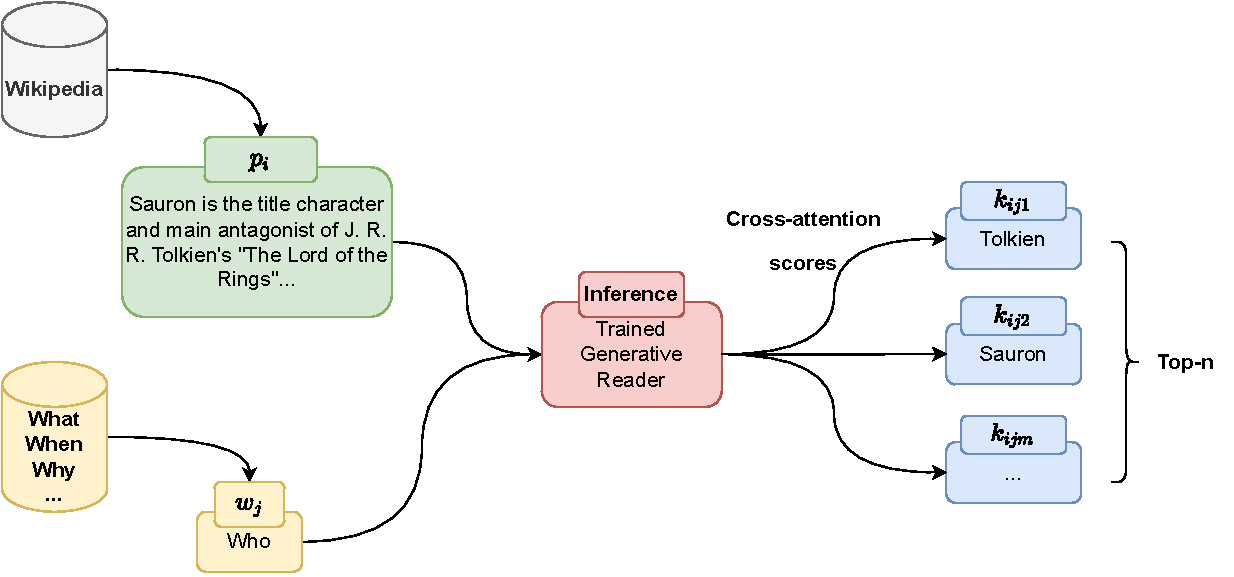
\includegraphics[width=0.95\linewidth]{query_expansion/unsupervised_keyword_extraction.pdf}
	\caption[Illustration of the unsupervised keyword extraction pipeline.]{
		%
		Illustration of the unsupervised keyword extraction pipeline.
		%
		For each passage $p_i$ in the Wikipedia corpus and each question type $w_j$, we generate a set of question-type-specific keywords $\{k_{ij1}, k_{ij2}, \ldots, k_{ijm}\}$ based on the cross-attention scores.
	}
	\label{fig:unsupervised_keyword_extraction_pipeline}
\end{figure}

%
In practice, we first analyze the Natural Questions dataset to obtain a set of commonly asked question types $\{w_1, w_2, \ldots\}$.
%
We then perform this unsupervised keyword extraction step on the entire Wikipedia corpus, obtaining a set of $m$ keywords $\{k_{ij1}, k_{ij2}, \ldots, k_{ijm}\}$ for each combination of passage $p_i$ and question type $w_j$, as illustrated in~\fref{fig:unsupervised_keyword_extraction_pipeline}.


\begin{figure}[!htbp]
	\centering
	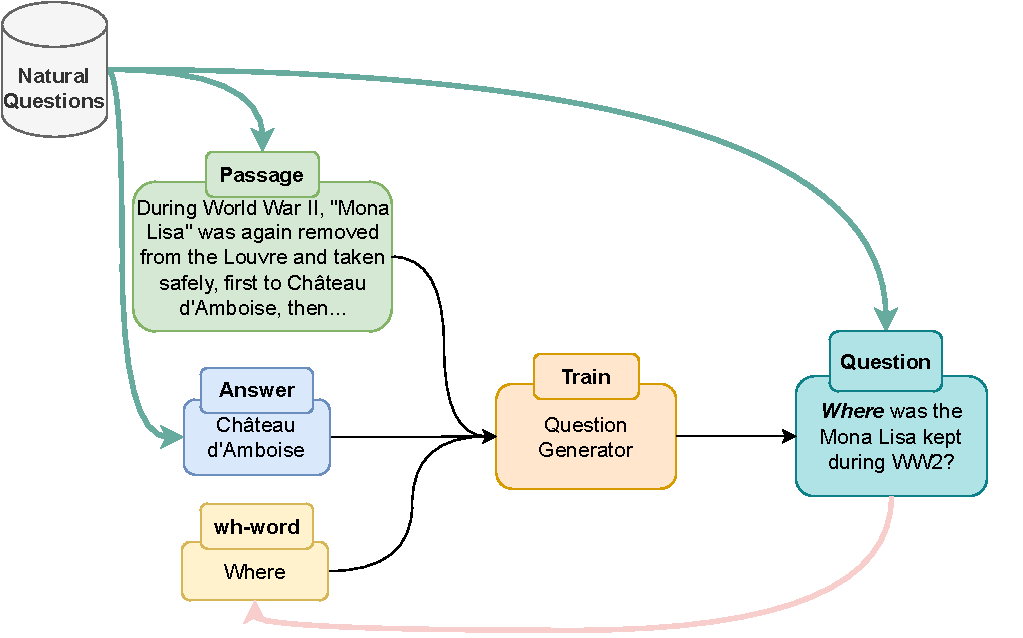
\includegraphics[width=0.8\linewidth]{query_expansion/question_generator_train.pdf}
	\caption[Illustration of the question generator training pipeline.]{
		%
		Illustration of the question generator training pipeline.
		%
		The model is trained to generate a plausible question given a context passage, an answer and a question type.
		%
		Different from existing work, we infer the question type from the questions use it as one of the supervised signals.
	}
	\label{fig:question_generator_train}
\end{figure}


\subsection{Question Generation}
\label{sec:question_generation_method}
%
Following existing work on synthetic question generation~\cite{alberti2019synthetic, chan2019recurrent, sultan2020importance, lewis2021paq}, we train a question generator model using supervised information from the Natural Questions dataset as shown in~\fref{fig:question_generator_train}.
%
However, we also provide the model with the question types of the target questions, thereby enhancing the capability of the model at generating plausible questions with an additionaly input signal, as well as more diverse questions with various question prompts.
%

\begin{figure}[!htbp]
	\centering
	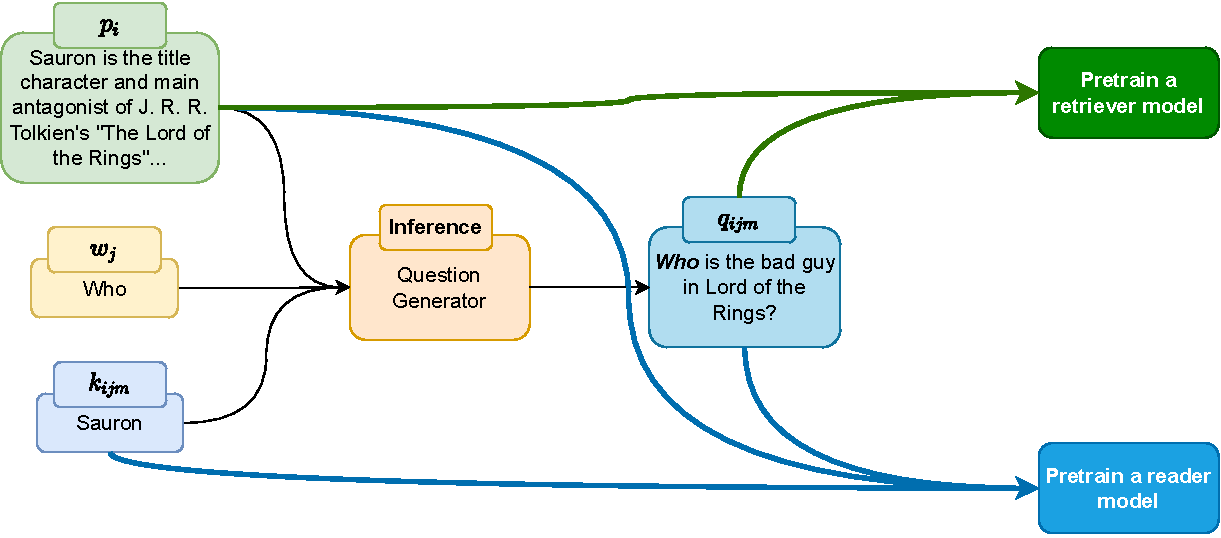
\includegraphics[width=\linewidth]{query_expansion/question_generator_inference.pdf}
	\caption[Illustration of the question generator inference pipeline.]{
		%
		Illustration of the question generator inference pipeline.
		%
		We take the trained question generator model to synthesize questions for passage-question type-keyword pairs obtained from the unsupervised keyword extraction step~\sref{sec:unsupervised_keyword_extraction}.
	}
	\label{fig:question_generator_inference}
\end{figure}

%
After finished, the trained question generator model will be used to infer a synthetic question $q_{ijm}$ for each combination of passage $p_i$, question type $w_j$ and keyword $k_{ijm}$ obtained from the unsupervised keyword extraction step~\sref{sec:unsupervised_keyword_extraction}.
%
This is illustrated in~\fref{fig:question_generator_inference}.
%
By doing so, we obtain an enormous, high-quality synthetic dataset of (passage $p_i$, question $q_{ijm}$, answer $k_{ijm}$) pairs.
%
This synthetic dataset can be used to pre-train both the retriever and reader model in the two-stage retriever-reader framework described in~\sref{sec:open_book}, following the procedure and conventions described in~\sref{sec:unsupervised_pre_training} in an unsupervised manner.

\subsection{Query Expansion}
\label{sec:query_expansion_submethod}



\begin{figure}[!ht]
	\centering
	
	\subfloat[Training]{%
		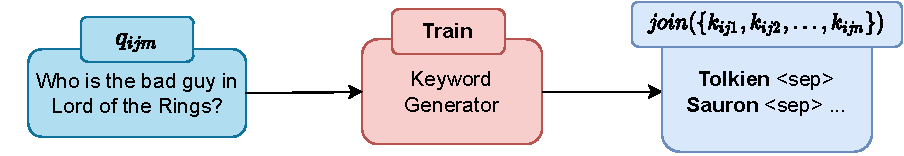
\includegraphics[clip,width=0.7\columnwidth]{query_expansion/query_expansion_method.pdf}%
	}
	\vspace{0.5cm}
	
	\subfloat[Inference]{%
		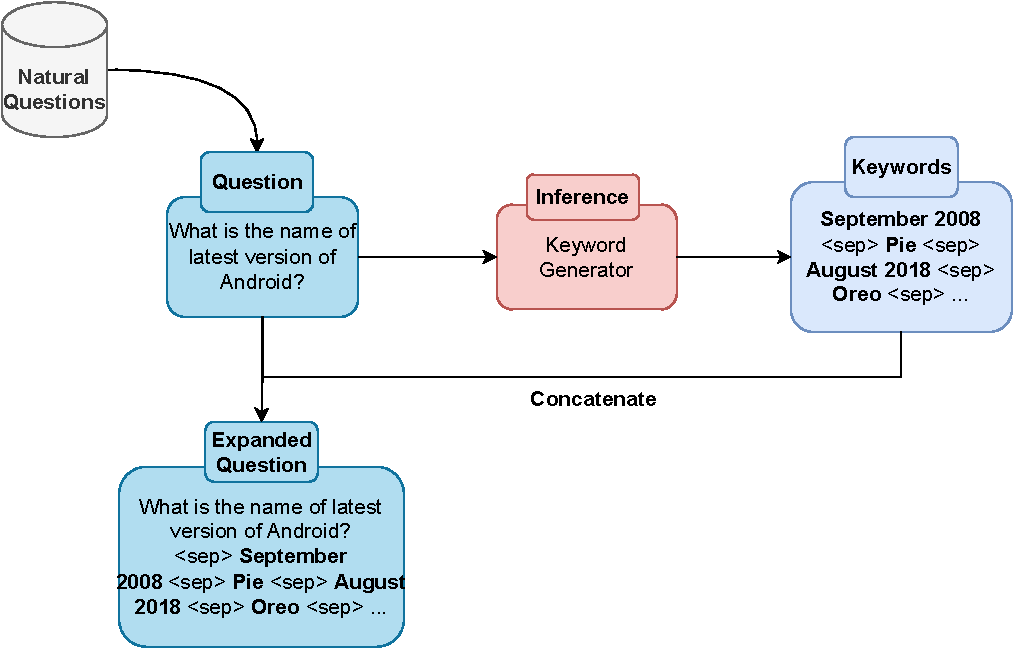
\includegraphics[clip,width=0.8\columnwidth]{query_expansion/query_expansion_method_inference.pdf}%
	}
	\caption[Illustration of the query expansion training and inference pipelines.]{
		%
		Illustration of the query expansion training and inference pipelines.
	}
	\label{fig:query_expansion_pipeline}
\end{figure}


The query expansion training and inference pipelines are illustrated in~\fref{fig:query_expansion_pipeline}.


\section{Experimental Results}
\label{sec:query_expansion_results}


We managed to implement and experiment with the processes of \emph{unsupervised keyword extraction} (\sref{sec:unsupervised_keyword_extraction}), \emph{question generation} (\sref{sec:question_generation_method}) as well as unsupervised retriever and reader pre-training (\sref{sec:question_generation_method}).

\begin{table*}[t!]
	\setlength\tabcolsep{5pt}
	\centering
	\small
	\begin{tabular}{ll|cc}
		\toprule
		\textbf{Architecture} & \textbf{Model}
		& Top-20 & Top-100 \\ 
		\midrule
		\multirow{3}{*}{\shortstack{DPR retriever~\cite{karpukhin2020dense}}} 
		& Original (real) & 78.4 & 85.4  \\
		& Pre-trained (synthetic) & 70.2 & 81.5 \\
		& Pre-trained (synthetic) + fine-tune (real) & \textbf{80.5} & \textbf{86.7} \\
		\bottomrule
	\end{tabular}
	\caption[Top-$\{20, 100\}$ retrieval accuracy on the Natural Questions test set of the DPR retriever with and without unsupervised pre-training.]{
		%
		Top-$\{20, 100\}$ retrieval accuracy on the Natural Questions test set of the DPR retriever with and without unsupervised pre-training
	}
	
	\label{tab:retriever_unsupervised_pretraining}
\end{table*}



\begin{table*}[t!]
	\setlength\tabcolsep{5pt}
	\centering
	\small
	\begin{tabular}{ll|c}
		\toprule
		\textbf{Architecture} & \textbf{Model}
		& Exact Match \\ 
		\midrule
		\multirow{3}{*}{\shortstack{DPR reader~\cite{karpukhin2020dense}}} 
		& Original (real) & 41.5  \\
		& Pre-trained (synthetic) & 28.4 \\
		& Pre-trained (synthetic) + fine-tune (real) & \textbf{44.4} \\
		\bottomrule
	\end{tabular}
	\caption[Top-$\{20, 100\}$ retrieval accuracy on the Natural Questions test set of the DPR reader with and without unsupervised pre-training.]{
		%
		Top-$\{20, 100\}$ retrieval accuracy on the Natural Questions test set of the DPR reader with and without unsupervised pre-training
	}
	
	\label{tab:reader_unsupervised_pretraining}
\end{table*}




\begin{table*}[t!]
	\setlength\tabcolsep{5pt}
	\centering
	\small
	\begin{tabular}{ll|c}
		\toprule
		\textbf{Architecture} & \textbf{Model}
		& Exact Match \\ 
		\midrule
		\multirow{3}{*}{\shortstack{FiD reader~\cite{izacard2021leveraging}}} 
		& Original (real) & 48.2  \\
		& Pre-trained (synthetic) & 32.8 \\
		& Pre-trained (synthetic) + fine-tune (real) & \textbf{49.8} \\
		\bottomrule
	\end{tabular}
	\caption[Top-$\{20, 100\}$ retrieval accuracy on the Natural Questions test set of the FiD reader~\cite{izacard2021leveraging} with and without unsupervised pre-training.]{
		%
		Top-$\{20, 100\}$ retrieval accuracy on the Natural Questions test set of the FiD reader with and without unsupervised pre-training
	}
	
	\label{tab:fid_reader_unsupervised_pretraining}
\end{table*}


The results are presented in~\tref{tab:retriever_unsupervised_pretraining},~\tref{tab:reader_unsupervised_pretraining} as well as~\tref{tab:fid_reader_unsupervised_pretraining}.